\documentclass[aspectratio=169]{beamer}

\usetheme{default}
\setbeamertemplate{navigation symbols}{}
\setbeamertemplate{enumerate item}{\color{navy}\arabic{enumi}.}
\setbeamertemplate{itemize item}{\color{black}\textbullet}
\setbeamertemplate{itemize subitem}{\color{black}\textbullet}
\usepackage{booktabs}
\usepackage{xcolor}
\usepackage{tikz}
\usetikzlibrary{shapes,arrows,positioning}
\definecolor{navy}{RGB}{0, 0, 128}
\definecolor{lightblue}{RGB}{230,240,250}
\definecolor{darkgreen}{RGB}{0,100,0}
\definecolor{lightgreen}{RGB}{230,250,230}
\newcommand{\highlight}[1]{\colorbox{lightblue}{$\displaystyle\textcolor{navy}{#1}$}}
\newcommand{\highlighttext}[1]{\colorbox{lightblue}{\textcolor{navy}{#1}}}
\newcommand{\highlightgreen}[1]{\colorbox{lightgreen}{$\displaystyle\textcolor{darkgreen}{#1}$}}

\usepackage{hyperref}
\hypersetup{
    colorlinks=true,
    linkcolor=navy,
    urlcolor=navy,
    citecolor=navy
}

\begin{document}


\begin{frame}
\centering
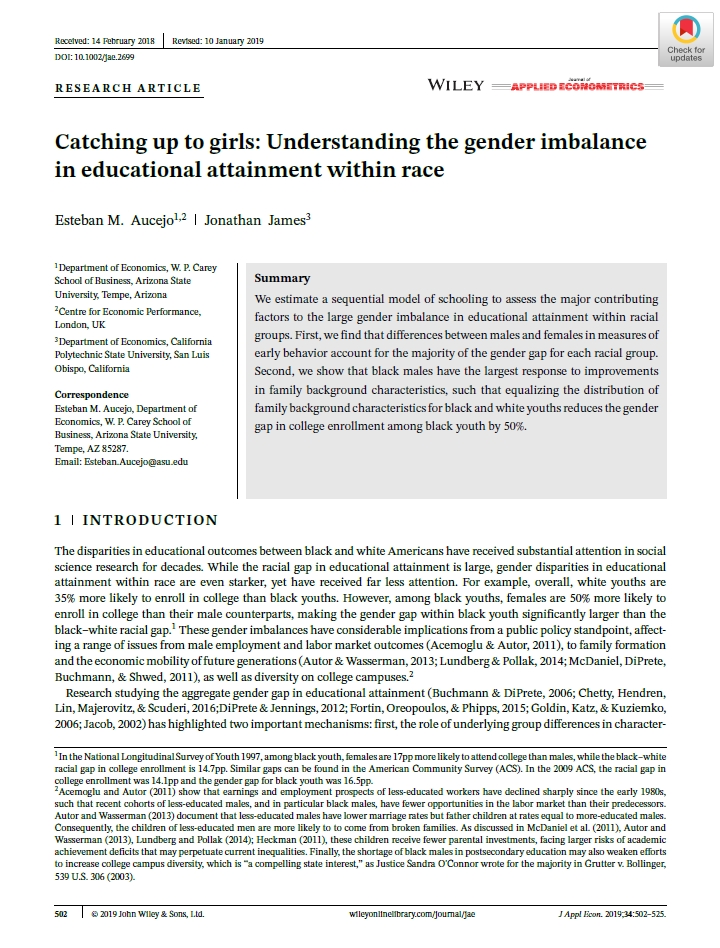
\includegraphics[width=0.5\textwidth]{Aucejo_James_2019_JAE_cover.jpg}
\end{frame}

\begin{frame}
\textcolor{navy}{Question:} Why are gender gaps in educational attainment larger \textit{within} racial groups than overall across racial groups?
\bigskip

\begin{itemize}
\itemsep1.5em
\item<2-> Extract 3 factors from 59 measures: family, math/verbal, behavior
\item<3-> Allow factor distributions to be extremely flexible (mixture of normals)
\item<4-> Model grade-by-grade decisions (10th grade $\to$ college)
\item<5-> Allow differential factor responses by race $\times$ gender $\times$ grade level
\end{itemize}
\end{frame}

\begin{frame}
\begin{itemize}
\itemsep1.5em
\item<1-> Use MM algorithm to estimate model
\item<2-> Use estimates to simulate effectiveness of policies that would narrow factor gaps
\item<3-> Find that Black men are uniquely responsive to family background: 
\bigskip\par
\begin{itemize}
    \item equalizing family factor for Blacks and Whites would reduce gender gap by 50\%
\end{itemize}

\end{itemize}
\end{frame}


\begin{frame}
\centering
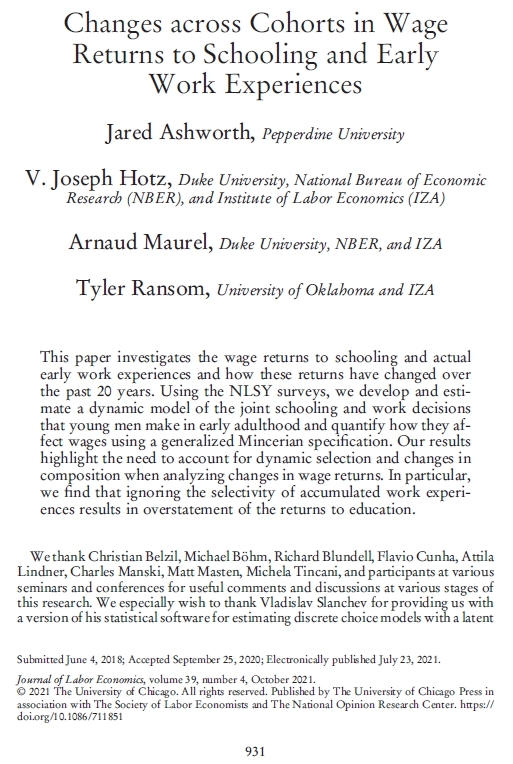
\includegraphics[width=0.4\textwidth]{Ashworth_al_2021_JOLE.jpg}
\end{frame}


\begin{frame}
\textcolor{navy}{Question:} How have wage returns to schooling/work experience changed over time?
\bigskip

\begin{itemize}
\itemsep1.5em
\item<2-> NLSY79 (born 1959-64) vs NLSY97 (born 1980-84)
\item<3-> Dynamic model: joint schooling \& work decisions ages 16-35
\item<4-> Distinguish work types: in-high-school, in-college, part-time, full-time
\item<5-> Control for selection: 2 unobserved factors (cognitive, noncognitive)
\item<6-> Noncognitive factor identified from panel data serial correlation
\end{itemize}
\end{frame}

\begin{frame}
\begin{itemize}
\itemsep1.5em
\item<1-> Use quadrature to integrate factors out of likelihood
\item<2-> Compare wage marginal effects w/ and w/out selection correction
\item<3-> Find that selection-corrected returns to college haven't gone up
\item<4-> Cognitive skill returns $\downarrow$ while Other skill returns $\uparrow$
\item<5-> Ignoring actual work experience $\Rightarrow$ overstates education returns
\end{itemize}
\end{frame}


\begin{frame}
\centering
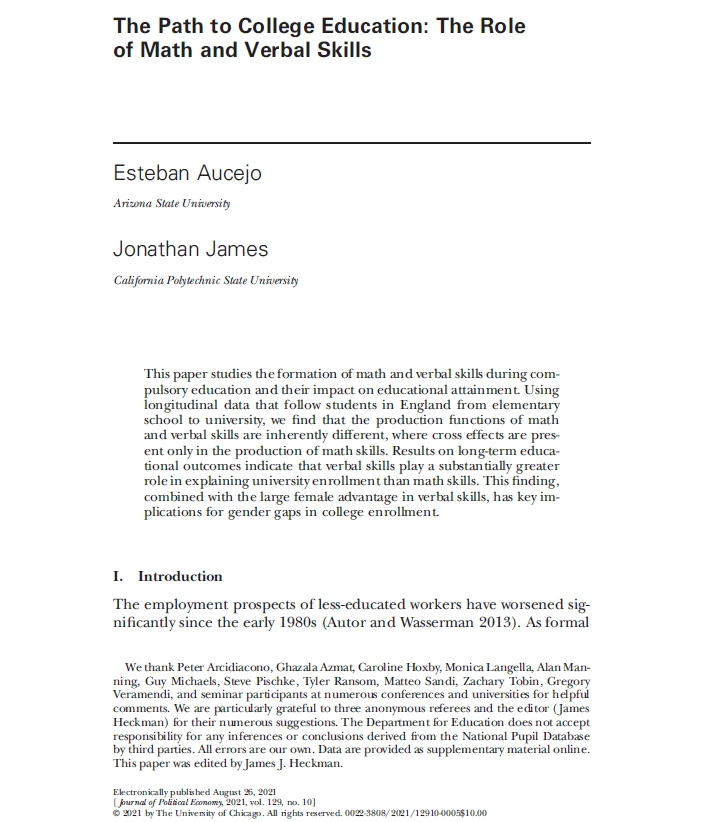
\includegraphics[width=0.5\textwidth]{Aucejo_James_2021_JPE_cover.jpg}
\end{frame}

\begin{frame}
\textcolor{navy}{Question:} How do math vs. verbal skills shape educational attainment in UK?
\bigskip

\begin{itemize}
\itemsep1.5em
\item<2-> Dynamic factor model: recover math/verbal skills across 4 Key Stages (ages 5-16)
\item<3-> Rich set of measurements: 30+ subject exams per student
\item<4-> Nested CES production function (3 inputs: past math, past verbal, school quality)
\item<6-> Account for selection into (elective) KS4 subjects via conditional logit
\end{itemize}
\end{frame}

\begin{frame}
\begin{itemize}
\itemsep1.5em
\item<1-> Use MM algorithm to estimate mixture of 10 normals for factor distributions
\item<2-> Find asymmetric cross-effects: verbal $\to$ math but not math $\to$ verbal
\item<3-> Verbal skills \textcolor{navy}{2-3x more important} than math for college enrollment
\item<4-> Female verbal advantage explains entire college enrollment gender gap
\item<5-> Counterfactual: universal high-quality schools $\Rightarrow$ +10\% college enrollment
\item<6-> U.S. validation (NLSY97): similar verbal $>$ math pattern for enrollment
\end{itemize}
\end{frame}


\begin{frame}
\centering
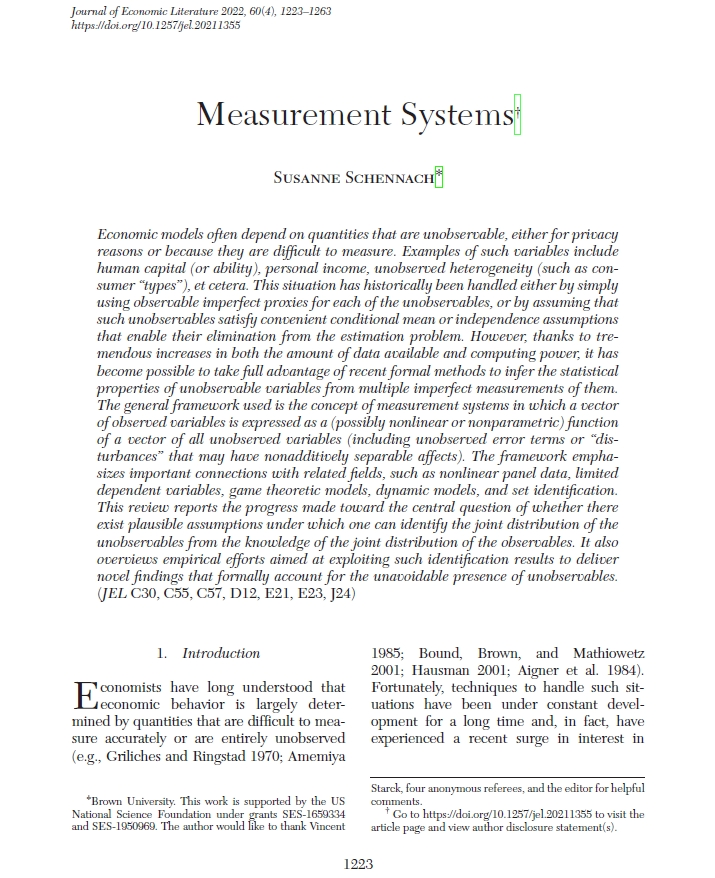
\includegraphics[width=0.5\textwidth]{Schennach_2022_JEL_cover.jpg}
\end{frame}

\begin{frame}
\textcolor{navy}{Question:} How can we identify distributions of unobservables from multiple imperfect measurements?
\bigskip

\begin{itemize}
\itemsep1.5em
\item<2-> General framework: measurement systems with vector of latent variables
\item<3-> Multidimensional settings: exploit common signal across measurements
\item<4-> Beyond classical assumptions: nonlinear, non-additive, non-zero-mean errors
\item<5-> Connections: factor models, panel data, limited dependent variables
\item<6-> Identification strategies when true values are entirely unobservable
\item<7-> Rich data $+$ computing power $\Rightarrow$ formally account for unobservables
\end{itemize}
\end{frame}



\end{document}